\documentclass[12pt, a4paper, oneside]{article}

\providecommand{\pgfsyspdfmark}[3]{}

% border setting
\usepackage[ top=2.5cm,bottom=2.5cm,left=2.5cm,right=2.5cm ]{ geometry }

% The default for LaTeX is to have no indent after sectional headings, like \chapter and \section. ()
\usepackage{indentfirst}

% http://tex.stackexchange.com/questions/28333/continuous-v-per-chapter-section-numbering-of-figures-tables-and-other-docume
% 讓圖片,表格編號自動連續編號
\usepackage{chngcntr}
\counterwithout{figure}{section}
\counterwithout{table}{section}

% This prevents placing floats before a section
\usepackage[section]{placeins}
\let\Oldsubsection\subsection
\renewcommand{\subsection}{\FloatBarrier\Oldsubsection}

% source code hightlighting
\usepackage{listings}
\lstset{
	numbers=left,
	stepnumber=1,
	firstnumber=1,
	captionpos=b,
	tabsize=2,
	basicstyle=\small,
	numberfirstline=true
}

\usepackage{graphicx}
\graphicspath{ {./figures/} }

% Insert watermark for each pages
\usepackage{background}
\backgroundsetup{
	contents={\includegraphics[]{ntut_watermark.jpg}},
	scale=0.2,
	opacity=0.4,
	angle=0
}

\usepackage[subpreambles=true]{standalone}

% setting the page number to footer
\usepackage{fancyhdr}
\fancyhf{}
\cfoot{\thepage}
\pagestyle{fancy}
% no header and footer bar
\renewcommand{\headrulewidth}{0pt}
\renewcommand{\footrulewidth}{0pt}

% line height setting
\linespread{1.5}
\usepackage{setspace}

\usepackage{xeCJK} %打中文必備
\setCJKmainfont{Noto Sans CJK TC} %設定中文字型,而英文不去更動

\usepackage{pdfpages}

\newcommand{\engUniversity}{National Taipei University of Technology}
\newcommand{\engDep}{Department of Computer Science and Information Engineering}
\newcommand{\courseName}{Mobile Robots}
\newcommand{\proposal}{proposal}

\newcommand{\englishTitle}{Obstacle Avoidance Using Dynamic Window Approach For Drone}

\newcommand{\studentEnName}{Pao-Hsun, Chen, and Yong-Jhen, Jheng}
\newcommand{\profEnName}{Huei-Yung Lin}

\newcommand{\dateEn}{April, 18, 2024}


\begin{document}
	\begin{titlepage}
	\begin{center}
		\LARGE
		\begin{singlespace}
			\textbf{\englishTitle{}} \\[0.5cm]
		\end{singlespace}
		
		\begin{singlespace}
			\begin{tabular}{r l}
				Student     & : \studentEnName{}  \\
				Advisor  & : Dr. \advisorEnName{} \\[0.5cm]
			\end{tabular}
		\end{singlespace}
		
		\begin{singlespace}
			Department of Computer Science
			and Information Engineering
			National Taipei University of Technology\\[0.5cm]
		\end{singlespace}
		
	\end{center}
\end{titlepage}
	
	\documentclass[crop=false]{standalone}
\begin{document}
	\section{Background}
	避開障礙物是自主移動式機器人在進行自主導航時一項基礎且必不可少的技術,無論是在工廠環境、室內環境、或是戶外環境下都是不可或缺的技能,使得這些機器人可以參與我們的日常生活以及工作。而且這樣的需求不斷在增長,例如:在餐廳中負責帶領客人前往桌位的機器人,在餐廳中負責送參的機器人,在居家環境裡負責清潔工作的機器人,在戶外環境下的自動駕駛汽車。這些機器人面臨一項共同的挑戰,需要避開動態和靜態的障礙物。動態障礙物包括行人,行進中的汽機車等等。靜態障礙物包括桌椅,貨物架,貨物等等。
	
	過去的研究已經提出了各種無人機避障方法,包括基於感測器的方法、視覺導航方法和軌跡規劃方法等。然而,這些方法在處理複雜的環境和動態的障礙物時仍然存在一定的挑戰,例如計算成本高、運算效率低、對環境變化敏感等。
	
	本文中採用的自主移動式機器人為四軸無人機,並且假設在室內環境下避開靜態障礙物。為了解決這個問題,我們使用基於Dynamic Window Approach (DWA)\cite{fox}解決方案動態調整機器人行進路線,使得機器人可以避開障礙物。
	
	DWA主要是用於局部路徑規劃,在本文中因為使用無人機,所以假設在固定高度下進行實驗,這使得問題可以簡化成在 2D 空間空的路徑規劃問題。DWA在速度空間中採集多組速度,並模擬機器人在這些速度下一定時間內的軌跡。在得到多組軌跡後,對這些軌跡比較,並且從中採取最佳軌跡所對應的速度來驅動機器人運動
\end{document}

	\newpage
	\documentclass[crop=false]{standalone}
\begin{document}
	\section{Background}
	Avoiding obstacles is a fundamental and essential technology for autonomous mobile robots when performing autonomous navigation. This skill is indispensable in environments such as factories, indoors, or outdoors, enabling these robots to participate in our daily lives and work. The demand for such capabilities is continually growing, for example, robots in restaurants that guide customers to their tables, deliver orders, robots in home environments responsible for cleaning, and autonomous vehicles outdoors. These robots face a common challenge: they need to avoid both dynamic and static obstacles. Dynamic obstacles include pedestrians and moving vehicles, while static obstacles include tables, chairs, racks, and goods.
	
	Past research has proposed various unmanned obstacle avoidance methods, including sensor-based methods, visual navigation, and trajectory planning. However, these methods still face certain challenges when dealing with complex environments and dynamic obstacles, such as high computational costs, low operational efficiency, and sensitivity to environmental changes.
	
	In this paper, we focus on a quadrotor drone as the autonomous mobile robot and assume it avoids static obstacles in an indoor environment. To address this issue, we use the Dynamic Window Approach (DWA) solution to dynamically adjust the robot's route to navigate around obstacles.
	
	DWA is primarily used for local path planning. In this paper, since we use drones, we assume experiments are conducted at a fixed height, simplifying the problem to a 2D space path planning issue. DWA collects multiple velocity sets in velocity space and simulates the robot's trajectory over a certain period at these velocities. After obtaining multiple sets of trajectories, we compare them and select the optimal trajectory's corresponding speed to drive the robot's motion.
\end{document}
	\newpage
	
	\documentclass[crop=false]{standalone}
\begin{document}
	\section{Methodology}
	\subsection{General Kinematics Model}
	本文實驗使用無人機,並且假設在固定高度下進行,這使得局部路徑規劃問題可以簡化成在2維空間上的路徑規劃問題。DWA 將機器人的位置控制問題轉成速度控制問題,並利用速度控制預測機器人運動軌跡。為此,需要先分析機器人運動模型\cite{fox},令$x(t), y(t)$為在$t$時間下,機器人的世界座標系下的位姿,且令機器人的方向為$\theta(t)$,則機器人運動可被表達為$<x, y, \theta>$,令機器人的平移速度為$v$,轉向加速度為$\omega(t)$,則一般來說可以表達如下:。
	
	\begin{equation}
		x(t_n)=x(t_0)+ \int_{t_0}^{t_n}v(t) \cdot cos(\theta)dt
	\end{equation}
	\begin{equation}
		y(t_n)=y(t_0)+ \int_{t_0}^{t_n}v(t) \cdot sin(\theta)dt
	\end{equation}
	\begin{equation}
		\theta(t)=\theta(t_0)+\int_{t_0}^{t_n}\omega(t)dt
	\end{equation}
	
	\subsection{Obstacle Avoidance}
	本文中障礙物為靜態障礙物,且每次隨機生成。在已知障礙座標下,可計算機器人與障礙物之間的距離$dist$,再加上安全距離$dist_{safe}$後可得到機器人避開的空間範圍,$dist$透過歐基里德公式計算後可得到,而安全距離則是根據經驗設置,本文中設定安全距離為5格
	
	\subsection{Cost Function}
\end{document}
	\newpage
	\documentclass[crop=false]{standalone}
\begin{document}
	\section{Methodology}
	\subsection{System Overview}
	The system architecture, as shown in Figure 1, begins with RGBD cameras capturing images with depth information. These RGB and depth images are then fed into the YOLO object detection model. The object detection task is performed by a deep learning model, which detects objects and provides their positions. These positions are then transformed into coordinates and used by the DWA for dynamic path adjustment. Additionally, a shortest path algorithm is incorporated to enhance the speed of path selection in DWA. This shortest path allows the drone to reach the specified location in minimal time while avoiding obstacles.
	
	\begin{figure*}[thbp!]
		\centering
		\fbox{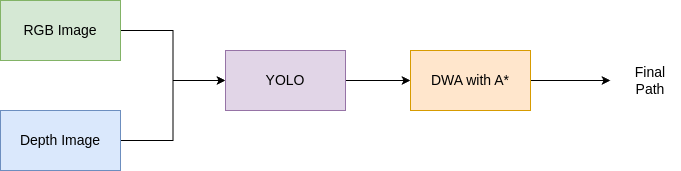
\includegraphics[width=\textwidth]{furtherwork_workflow}}
		\caption{The system architecture}
		\label{fig:system}
	\end{figure*}
	
	\subsection{General Kinematics Model}
	This study utilizes drones and assumes motion at a fixed altitude and speed, simplifying local path planning problems into 2D path planning problems. DWA transforms the robot's position control problem into a velocity control problem and predicts the robot's motion trajectory through velocity control. To achieve this, the robot's motion model needs to be analyzed \cite{fox}. Let $x(t), y(t)$ denote the robot's pose in the world coordinate system at time $t$, and let $\theta(t)$ represent the direction of the robot. Thus, the robot's motion can be expressed as $<x, y, \theta>$. Let $v$ denote the translational velocity of the robot and $\omega(t)$ denote the angular acceleration. Generally, this can be expressed as follows:
	\begin{equation}
		x(t_n)=x(t_0)+ \int_{t_0}^{t_n}v(t) \cdot cos(\theta)dt
	\end{equation}
	\begin{equation}
		y(t_n)=y(t_0)+ \int_{t_0}^{t_n}v(t) \cdot sin(\theta)dt
	\end{equation}
	\begin{equation}
		\theta(t)=\theta(t_0)+\int_{t_0}^{t_n}\omega(t)dt
	\end{equation}
	\subsection{Objective Function}
	Due to the presence of multiple different translational velocities and angular velocities, it is necessary to select the optimal path from the paths formed by different combinations of translational velocities and angular velocities. The selection process is based on the following objective function:
	\begin{equation}
		G(v, \omega)=\sigma(\alpha Heading(v, \omega) + \beta Obstacle(v, \omega) + \gamma Velocity(v, \omega))
	\end{equation}
	\begin{itemize}
		\item Heading function - This function is used to ensure that the robot advances towards the destination while maintaining its orientation towards it. A smaller value of $\theta$ indicates that the angle between the robot and the destination is smaller.
		\item Obstacle avoidance function - In this study, obstacles are static and generated randomly each time. Given the coordinates of the obstacles, the distance $dist$ between the robot and the obstacle can be calculated using the Euclidean formula. If the distance between the robot and the obstacle is greater than the radius of the robot, it can be considered as no collision occurring.
		\item Velocity function - The translation speed of the robot
	\end{itemize}
	$\sigma$ 
	The function is then normalized across the three functions.
	\begin{equation}
		normalHead(i)=\frac{head(i)}{\sum_{i=1}^{n}{head(i)}}
	\end{equation}
	\begin{equation}
		normalDist(i)=\frac{dist(i)}{\sum_{i=1}^{n}{dist(i)}}
	\end{equation}
	\begin{equation}
		normalVelocity(i)=\frac{velocity(i)}{\sum_{i=1}^{n}{velocity(i)}}
	\end{equation}
	Here, n represents all sampled trajectories, and i denotes the current trajectory being evaluated.
\end{document}
	\newpage
	
	\documentclass[crop=false]{standalone}

\begin{document}
	\section{Expected Result}
	本文實驗假設無人機在固定高度,固定速度下前進,並且給定三個參數,1) 給定無人機初始座標位置,2) 給定終點目標 3)隨機生成多個障礙物後,將障礙物位置當成第二個輸入參數。我們預期在獲得輸入參數後,無人機起飛後會首先調整前進方向,由於本文假設無人機以固定速度前進,只需要持續計算與障礙物的距離,並且與障礙物保持安全距離,以及調整方向在並避開障礙物的同時也保持朝向終點方向前進。總結來說,我們預期透過使用DWA方法,無人機將能夠避開障礙物,並以穩定的速度行向自目的地, 如圖1所示:
    
    \begin{figure}[htbp]	
    	\centering
    	\begin{minipage}{0.49\linewidth}
    		\centering
    		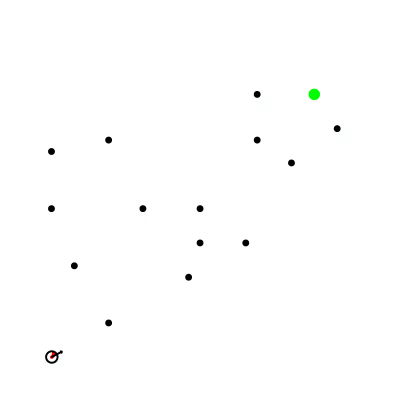
\includegraphics[width=0.9\linewidth]{dwa_frame_0.png}
    		\caption{Initial point}
    		\label{Initial robot point}%文中引用该图片代号
    	\end{minipage}
    	\begin{minipage}{0.49\linewidth}
    		\centering
    		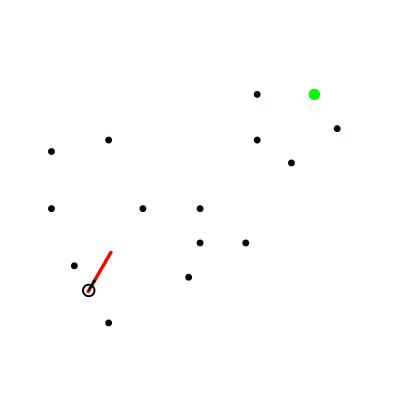
\includegraphics[width=0.9\linewidth]{dwa_frame_1.png}
    		\caption{Robot is moving}
    		\label{Moving robot}%文中引用该图片代号
    	\end{minipage}
    	%\qquad
    	%让图片换行,
    	
    	\begin{minipage}{0.49\linewidth}
    		\centering
    		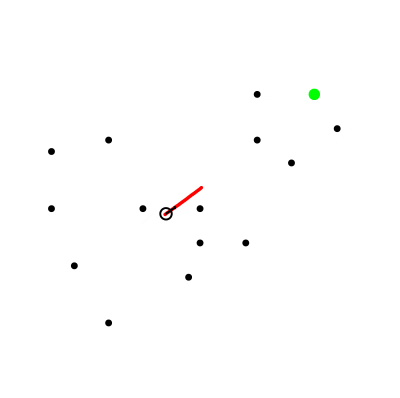
\includegraphics[width=0.9\linewidth]{dwa_frame_2.png}
    		\caption{Robot avoid obstacles}
    		\label{Robot avoid obstacles}%文中引用该图片代号
    	\end{minipage}
    	\begin{minipage}{0.49\linewidth}
    		\centering
    		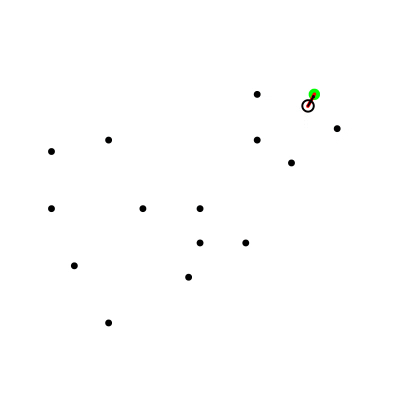
\includegraphics[width=0.9\linewidth]{dwa_frame_3.png}
    		\caption{Robot is arrived target point}
    		\label{Robot is arrived target point}%文中引用该图片代号
    	\end{minipage}
    \end{figure}
\end{document}


	\newpage
	\documentclass[crop=false]{standalone}
\begin{document}
	\section{Expected Result}

\end{document}
	\newpage
	
	
	\begin{thebibliography}{1}
		
		\bibitem{fox}
		D. Fox, W. Burgard and S. Thrun, The dynamic window approach to collision avoidance," in IEEE Robotics \& Automation Magazine, vol. 4, no. 1, pp. 23-33, March 1997, doi: 10.1109/100.580977. keywords: {Collision avoidance;Mobile robots;Robot sensing systems;Orbital robotics;Robotics and automation;Motion control;Humans;Robot control;Motion planning;Acceleration},
		
		\bibitem{missura}
		M. Missura and M. Bennewitz, "Predictive Collision Avoidance for the Dynamic Window Approach," 2019 International Conference on Robotics and Automation (ICRA), Montreal, QC, Canada, 2019, pp. 8620-8626, doi: 10.1109/ICRA.2019.8794386.
		keywords: {Trajectory;Vehicle dynamics;Dynamics;Acceleration;Collision avoidance;Robot sensing systems},
		
		\bibitem{carrio}
		A. Carrio, J. Tordesillas, S. Vemprala, S. Saripalli, P. Campoy and J. P. How, "Onboard Detection and Localization of Drones Using Depth Maps," in IEEE Access, vol. 8, pp. 30480-30490, 2020, doi: 10.1109/ACCESS.2020.2971938.
		keywords: {Drones;Three-dimensional displays;Feature extraction;Object detection;Sensors;Training;Cameras;Drone;detection;collision avoidance;depth map},
		
		\bibitem{devos}
		A. Devos, E. Ebeid and P. Manoonpong, "Development of Autonomous Drones for Adaptive Obstacle Avoidance in Real World Environments," 2018 21st Euromicro Conference on Digital System Design (DSD), Prague, Czech Republic, 2018, pp. 707-710, doi: 10.1109/DSD.2018.00009. keywords: {Drones;Collision avoidance;System recovery;Laser radar;Navigation;Signal processing algorithms;Propellers;Autonomous drone system;Adaptive obstacle avoidance;Simulation;Implementation},
		
		\bibitem{tordesillas}
		J. Tordesillas, B. T. Lopez, M. Everett and J. P. How, "FASTER: Fast and Safe Trajectory Planner for Navigation in Unknown Environments," in IEEE Transactions on Robotics, vol. 38, no. 2, pp. 922-938, April 2022, doi: 10.1109/TRO.2021.3100142.
		keywords: {Trajectory;Safety;Resource management;Optimization;Planning;Aerospace electronics;Hardware;Convex decomposition;path planning;trajectory optimization;UAV},
		
		
	\end{thebibliography}
	
\end{document}
